%----------------------------------------------------------------------------------
% Exemplo do uso da classe pucrs-ppgcc.cls. Veja o arquivo .cls
% para mais detalhes e instruções.
%----------------------------------------------------------------------------------
\chapter{\label{chap:intro}Introdução }
% Comando para inserir siglas. Tanto as siglas quanto as
% abreviaturas devem aparecer em ordem ALFABÉTICA nas listas
% correspondentes. Como a classe no momento não é capaz de ordenar
% as entradas automaticamente, existem duas alternativas:
%
%    a- Insira todas as siglas e abreviaturas no começo do texto,
%    manualmente e em ordem alfabética.
%
%    b- Caso esteja em um ambiente UNIX (Linux, Mac ou Cygwin/similares),
%    utilize o script sort.sh e o makefile que acompanham a
%    classe. O makefile automaticamente compila a monografia para
%    PDF (mas assume que o latex está acessível pela linha de
%    comando). Neste caso a ordenação é feita de forma automática.
%
\sigla{abc}{Associação Brasileira de Computadores}
\sigla{xyz}{lorem ipsum dolor sit}
\sigla{ijk}{lorem ipsum dolor sit}
%
% Comando para inserir abreviaturas.
%
\abrev{Abrev}{Abreviatura}
\abrev{Inform}{Informática}
%
% Comando para inserir símbolos. Estes irão aparecer em ordem
% de ocorrência, já que o número da página está presente na lista
% de símbolos.
\simbolo{Hz}{Hertz}
\simbolo{$\pi$}{Constante com valor aproximado de $3.1415926$}%
%
lorem ipsum dolor sit amet Capítulo~\ref{chap:intro} consetetur
sadipscing elitr sed diam nonumy eirmod tempor invidunt ut labore
et dolore magna aliquyam erat sed diam voluptua at vero eos et
accusam et justo duo dolores et ea rebum stet clita kasd gubergren
no sea takimata sanctus est lorem ipsum dolor sit amet lorem ipsum
dolor sit amet consetetur sadipscing elitr sed diam nonumy eirmod.
Ver Figura~\ref{fig:fig1}.

% Um exemplo de figura
\begin{figure}[htb!]
\centering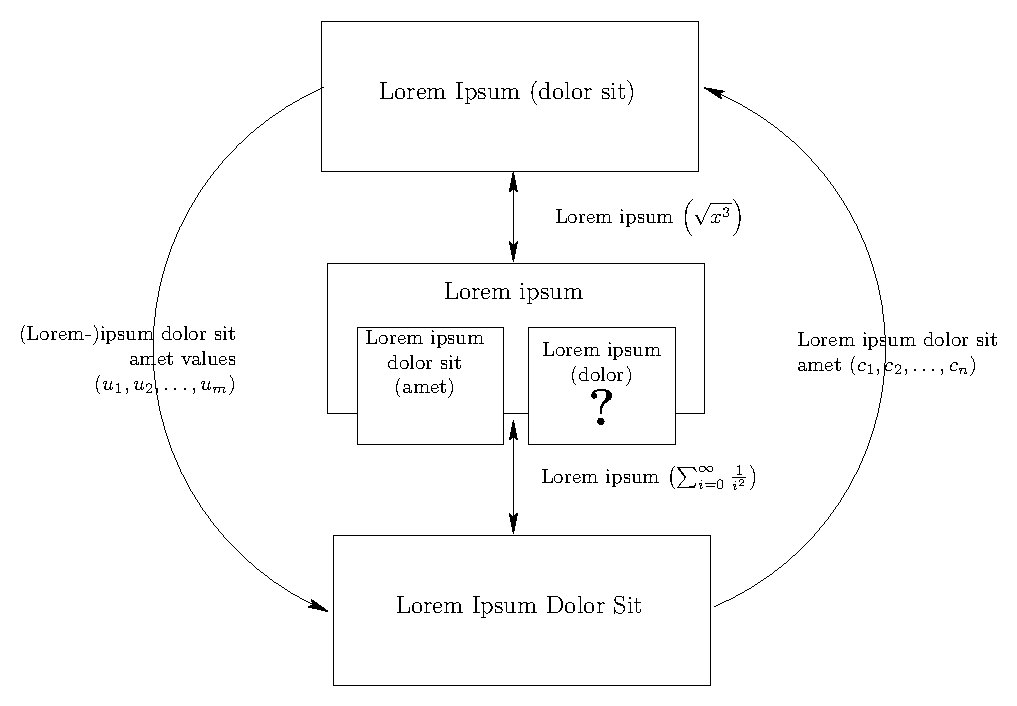
\includegraphics[width=.65\textwidth]{fig/exemplo.eps}
\caption%[This figure has a shorter caption now]%
        {\label{fig:fig1}This is a figure with a very long
    caption which looks ugly in the corresponding list of figures.
    Fortunately, there is an optional parameter for a shorter
    replacement of this monstrosity}%
\end{figure}

tempor invidunt~\cite{SKIENAC698} ut labore et dolore magna
aliquyam erat sed diam voluptua at vero eos et accusam et justo
duo dolores et ea rebum stet clita kasd gubergren no sea takimata
sanctus est lorem ipsum dolor sit amet lorem
ipsum~\cite{NAGAPACKING07}. O Algoritmo~\ref{alg:alg1}
mostra este processo.

\begin{algorithm}[htb]
\begin{center}
    % Um exemplo de algoritmo utilizando a pacote 'algorithmic'
    %\algsetup{linenosize=\small,linenodelimiter=.}
    \begin{algorithmic}[1]
        \STATE \textbf{function} $\sigma\left(i,j\right)$
        \STATE \COMMENT{\texttt{table} lorem ipsum dolor consetetur sadipscing elitr sed $\left(i,j\right)$}
        \IF{$\text{table}\left[i,j\right].\text{memoized}$}
            \RETURN $\text{table}\left[i,j\right].\text{error}$
        \ENDIF
        \STATE $\text{minerror}\leftarrow\infty$
        \STATE $\text{bestt}\leftarrow{}\text{nil}$
        \FOR { each template $t$ in $T$ }
            \STATE $\text{error}\leftarrow{}\text{allocate}\left(t,i,j\right)$
            \IF{$\text{error}<\text{minerror}$}
                \STATE $\text{minerror}\leftarrow{}\text{error}$
                \STATE $\text{bestt}\leftarrow{}t$
            \ENDIF
        \ENDFOR
        \STATE $\text{table}\left[i,j\right].\text{memoized}\leftarrow{}\text{true}$
        \STATE $\text{table}\left[i,j\right].\text{template}\leftarrow{}\text{bestt}$
        \STATE $\text{table}\left[i,j\right].\text{error}\leftarrow{}\text{minerror}$
        \RETURN $\text{minerror}$
    \end{algorithmic}
\end{center}
\caption[An algorithm with an optional, shorter caption]%
    {\label{alg:alg1}This is an algorithm with a very long
    caption. However, we replaced it with a shorter version
    in the Outline for legibility reasons}%
\end{algorithm}

tempor invidunt ut labore et dolore magna aliquyam erat sed diam
voluptua at vero eos et accusam et justo duo dolores et ea
rebum~\cite{CORMEMALGORITHMS01}.

dolor sit~\cite{BENTLEYBC07} amet consetetur sadipscing elitr sed
diam nonumy eirmod tempor invidunt ut labore et dolore magna
aliquyam erat sed diam voluptua at vero~\cite{BRIANPL04}.

\begin{enumerate}
   \item lorem
   \item ipsum
   \item dolor
   \item sit
   \item amet
   \item consetetur
\end{enumerate}

\section{\label{sec:secao1}História dos Sistemas de Tempo Real}

lorem ipsum dolor sit $x\leq 2$  amet consetetur sadipscing elitr
sed diam nonumy eirmod Seção~\ref{sec:secao1} tempor invidunt ut
labore et dolore magna aliquyam erat sed diam voluptua at vero eos
et accusam et justo duo dolores et ea rebum stet
clita.~\cite{OLIVEIRAAPL08}

% Um exemplo de fórmula
\begin{equation}\label{eq:eq1}
    \intop_{0}^{\infty}{x^2 + \frac{\pi}{\sum_{i=0}^{n}{\frac{1}{i^2}}}}
\end{equation}

kasd gubergren no sea Equação~\eqref{eq:eq1} takimata sanctus est
lorem ipsum dolor sit amet lorem ipsum dolor sit amet consetetur
sadipscing elitr sed diam nonumy eirmod.~\cite{PICCOLIAPL11}

amet lorem ipsum dolor sit amet consetetur sadipscing elitr sed
diam nonumy eirmod.~\cite{PICCOLIDM08}

\section{\label{sec:secao2}Tempo}
\subsection{Tempo na Execução}
\subsection{Tempo Lógico}
\subsection{Tempo Denso}
\subsection{Tempo Global}
\subsection{Tempo Absoluto}
\subsection{Tempo Relativo}


\section{\label{sec:secao3}Definição de um Sistema de Tempo Real}
\subsection{Aplicações}
\subsection{Problemas clássicos de tempo real}

\section{\label{sec:secao3}Tipos de Sistema de Tempo Real}
\subsection{Críticos}
\subsection{Não críticos}

\section{\label{sec:secao4}Tipos de escalonamentos}
\subsection{Rate monotonic scheduling}
\subsection{Round-Robin}
\subsection{Fixed-Priority}
\subsection{Critical section preemptive scheduling}
\subsection{Static time scheduling}
\subsection{Earliest Deadline First}
\subsection{Cooperative scheduling}

\section{\label{sec:secao5}Avaliação e garantias}
\subsection{Testes}
(Software Engineering: A Practitioner's Approach by Roger S Pressman)
\subsubsection{Teste de tarefas}
\subsubsection{Teste de comportamento}
\subsubsection{Teste intertarefa}
\subsubsection{Teste do sistema}

\subsection{Formalismo em análise de Sistemas de tempo real}
\subsubsection{Metodos de modelagem}
\subsubsection{Uso na indústria}
\subsubsection{Métodos Formais para verificação de sistemas}
\subsubsection{Ferramentas para verificação formal}



lorem ipsum dolor sit amet consetetur sadipscing elitr sed diam nonumy
eirmod tempor invidunt ut labore et dolore magna aliquyam erat sed diam
voluptua at vero eos et accusam et justo duo dolores et ea rebum
stet clita.~\cite{GOLDENBERGAPL02}

\begin{equation}\label{eq:apl}%
    L\left(i,j,w,h\right)=
    \begin{cases}
      E\left(i,w,h\right) & i=j\\
      \min\left(\min_{k=i}^{j-1}\left\{\heartsuit\left(i,k,j,w,h\right)\right\},
                \min_{k=i}^{j-1}\left\{\spadesuit\left(i,k,j,w,h\right)\right\}\right) & i<j\text{.}
    \end{cases}
\end{equation}

lorem ipsum dolor sit amet consetetur sadipscing elitr sed diam nonumy
eirmod tempor invidunt ut labore et dolore magna aliquyam erat sed diam
voluptua at vero eos et accusam et justo duo dolores et ea rebum stet clita
kasd gubergren no sea takimata sanctus est lorem ipsum dolor sit amet lorem
ipsum dolor sit amet consetetur sadipscing elitr sed diam nonumy eirmod
tempor invidunt ut labore et dolore magna aliquyam erat sed diam voluptua at
vero eos et accusam et justo duo dolores et ea rebum stet clita kasd
gubergren no sea takimata sanctus est lorem ipsum dolor sit amet lorem ipsum
dolor sit amet consetetur sadipscing elitr sed diam nonumy eirmod tempor
invidunt ut labore et dolore magna aliquyam erat sed diam voluptua at vero
eos et accusam et justo duo dolores et ea rebum stet clita kasd gubergren no
sea takimata sanctus est lorem ipsum dolor sit amet.

%----------------------------------------------------------------------------------
% Exemplo do ambiente para citações diretas com mais de 3 linhas.
%
% Para citações diretas de até 3 linhas, faça assim:
% De acordo com Direto~(2011, p.~21): "bla bla bla, bla 'bla'."
De acordo com Esquedo~(2011, p.~19):

\begin{directcite}
ut wisi enim ad minim veniam quis nostrud exerci tation ullamcorper suscipit
lobortis nisl ut aliquip ex ea commodo consequat duis autem vel eum iriure
dolor in hendrerit in vulputate velit esse molestie consequat vel illum
dolore eu feugiat nulla facilisis at vero eros et accumsan et
iusto odio
\end{directcite}

duis autem vel eum iriure dolor in hendrerit in vulputate velit esse
molestie consequat vel illum dolore eu feugiat nulla facilisis at vero eros
et accumsan et iusto odio dignissim qui blandit praesent luptatum zzril
delenit augue duis dolore te feugait nulla facilisi lorem ipsum dolor sit
amet consectetuer adipiscing elit sed diam nonummy nibh euismod tincidunt ut
laoreet dolore magna aliquam erat volutpat.

ut wisi enim ad minim veniam quis nostrud exerci tation ullamcorper suscipit
lobortis nisl ut aliquip ex ea commodo consequat duis autem vel eum iriure
dolor in hendrerit in vulputate velit esse molestie consequat vel illum
dolore eu feugiat nulla facilisis at vero eros et accumsan et iusto odio
dignissim qui blandit praesent luptatum zzril delenit augue duis dolore te
feugait nulla facilisi.

nam liber tempor cum soluta nobis eleifend option congue nihil imperdiet
doming id quod mazim placerat facer possim assum lorem ipsum dolor sit amet
consectetuer adipiscing elit sed diam nonummy nibh euismod tincidunt ut
laoreet dolore magna aliquam erat volutpat ut wisi enim ad minim veniam quis
nostrud exerci tation ullamcorper suscipit lobortis nisl ut aliquip ex ea
commodo consequat.
